The HACC framework arose from the early realization that development
of a future large-scale computational framework must be fully
cognizant of coming changes in computational architectures. It is
descended from an approach developed for the heterogeneous
architecture of Roadrunner~\cite{mc3,pope10}, the first computer to
break the petaflop barrier. HACC is designed with
great flexibility in mind (combining MPI with a variety of more local
programming models, e.g., OpenCL, OpenMP) and is easily adaptable to
different platforms. Currently, it is implemented on Cell-accelerated
hardware, conventional and GPU-enhanced clusters (via OpenCL), on the
IBM Blue Gene architecture (using OpenMP), and is running on prototype
Intel MIC/Xeon Phi hardware. HACC is the first, and currently the only
large-scale cosmology code suite world-wide, that can run at scale
(and beyond) on all available supercomputer
architectures. Figure~\ref{hacc_scale} shows the scaling on the entire
IBM BG/Q Sequoia up to 1,572,864 cores with an equal number of MPI
ranks, attaining 13.94 PFlops at 69.2\% of peak and 90\% parallel
efficiency -- this is the highest performance yet attained by a
science code on any computer; for details, see
Ref.~\cite{habib12}. Examples of science results obtained using HACC
include 64-billion particle runs for baryon acoustic oscillations
predictions for the BOSS Lyman-$\alpha$ forest~\cite{boss_bao} and
high-statistics predictions for the halo profiles of massive
clusters~\cite{conc_hacc}. Currently, a very large 1.1 trillion
particle simulation is being carried out on the BG/Q system Mira at
Argonne.  A nested snapshot at an early output time ($z\sim3$) from
this simulation is shown in Fig.~\ref{simpic}.

%FIXME --- Make sure correctly set up
\begin{figure}
  \centering 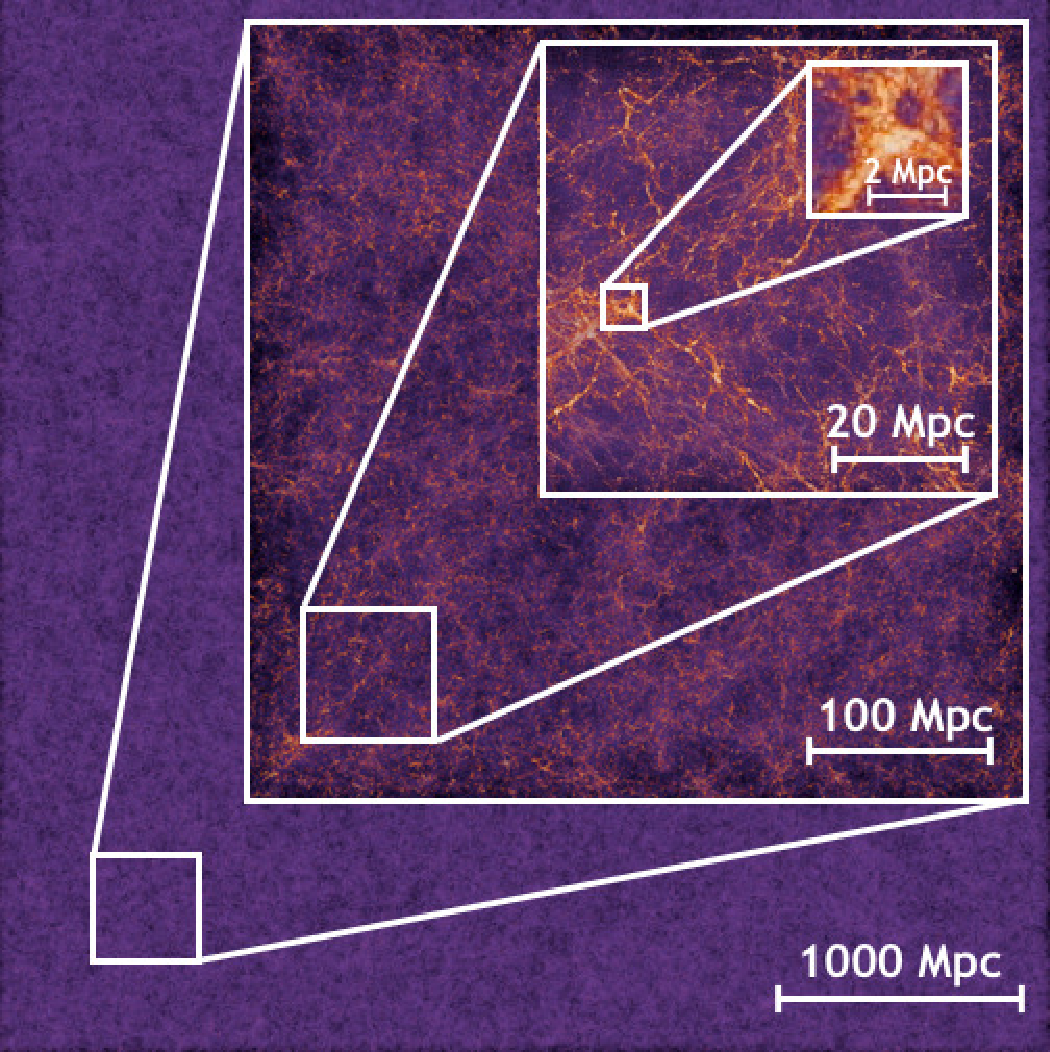
\includegraphics[width=0.5\columnwidth]{../Plots/zoom_in}
\caption{HACC result: Zoom-in visualization of the density
    field in a 1.1 trillion particle, 4.2~Gpc box size simulation with
    HACC on 32 BG/Q racks.  This figure illustrates the global
    dynamic range covered by the simulation, $\sim 10^6$, although the
    finer details are not resolved by the visualization.}
\label{simpic}
\end{figure}



HACC uses a hybrid parallel algorithmic structure, splitting the force
calculation into a specially designed grid-based long/medium range
spectral particle-mesh (PM) component that is common to all
architectures, and an architecture-specific short-range
solver. Modular code design combined with particle caching allows the
short-range solvers to be `hot-swappable' on-node; they are blind to
the parallel implementation of the long-range solver. 
The short-range solvers can use direct particle-particle interactions, i.e., a P$^3$M
algorithm~\cite{hockney}, as on Roadrunner or Titan, or use tree
methods as on the IBM BG/Q and Cray XE6 systems (TreePM
algorithm). The availability of multiple algorithms within the HACC
framework allows us to carry out careful error analyses, for example,
the P$^3$M and the TreePM versions agree to within $0.1\%$ for the
nonlinear power spectrum test in the code comparison suite of
Ref.~\cite{heitmann05}.

The HACC philosophy is that, as a general rule, both particle and grid
methods are difficult to implement as global solutions: For physics
and implementation reasons, grid-based techniques are better suited to
larger length scales, with particle methods having the opposite
property. This suggests that the higher `top' levels of code
organization should be grid-based, interacting with particle
information at a lower level of the computational hierarchy. The
design ideas underlying HACC give us a very important head start in
tackling the challenges posed by future architectures.

%FIXME --- Make sure correctly set up
\begin{figure}
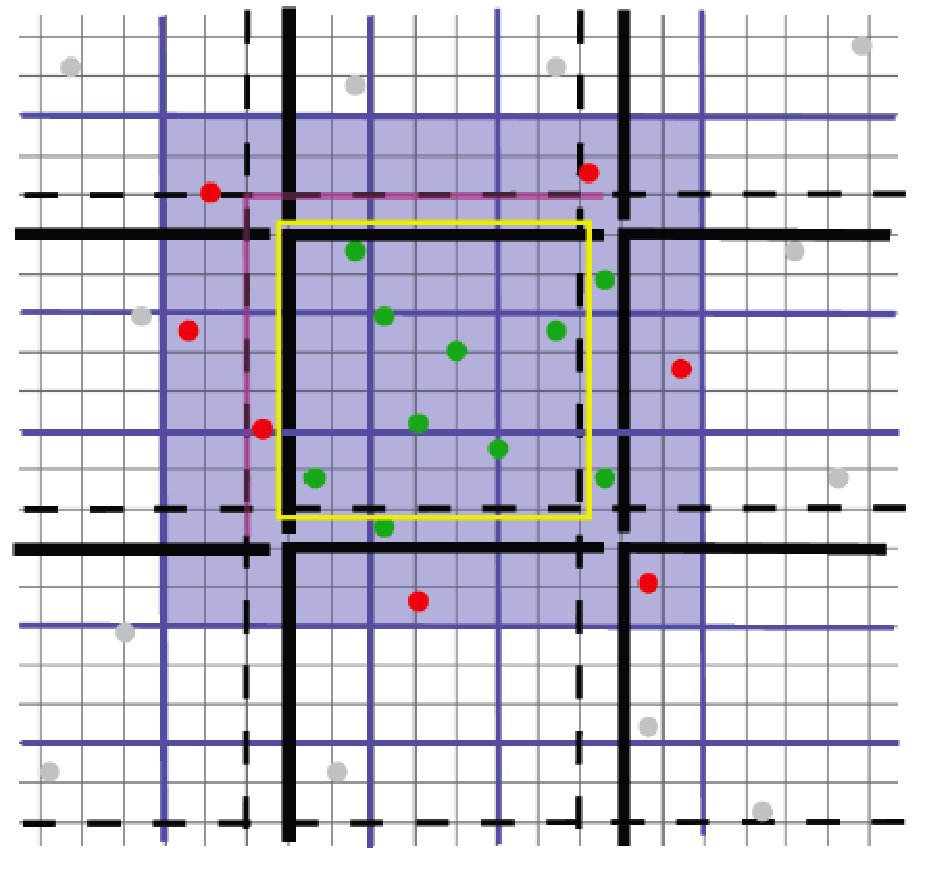
\includegraphics[width=0.5\columnwidth]{../Plots/overload}
\caption{ Overloading in a 2-D domain decomposition: A node
    holds particles within its domain (green) and particle copies out
    to a given distance from its boundary (red, in blue
    square). Copies held by neighboring nodes form a mirrored particle
    cache.}
\label{overload}
\end{figure}
\noindent



On heterogeneous systems such as Roadrunner, or Titan at Oak Ridge,
HACC has the following layout: At the top level, the medium/long range
force is handled by a special low-noise, high accuracy, FFT-based
method that operates at the CPU layer. Depending on the memory balance
between the CPU and the accelerator (Cell or GPU), we can choose to
specify two different modes, (i) grids held on the CPU and particles
on the accelerator, or (ii) a streaming paradigm with grid and
particle information primarily resident in CPU memory with
computations streamed through the accelerator. In both cases, the
local force solve is a direct particle-particle interaction, i.e., the
whole is a P$^3$M code~\cite{hockney} with hardware acceleration,
albeit an unconventional implementation based on high-order spectral
methods. The acceleration leads to a speed-up of 50-100 times over
conventional processors.  For a many-core system, the top layer of the
code remains the same, but the short-range solver changes to a
tree-based algorithm which is much better suited to the Blue Gene and
Intel MIC architectures.

Our strategy simultaneously overcomes two problems: (i) how to switch
short-range solvers easily, and (ii) overcome the communication
bottleneck between the CPU and accelerator layers, or the analog for a
many-core system (on-node vs. off-node communication). We drastically
reduce the particle communication by using a mirrored particle cache,
termed `particle overloading', implemented on top of our 3-D domain
decomposition (see Fig.~\ref{overload}). The point of overloading --
loosely analogous to ghost regions in mesh-based codes -- is to allow
exact medium/long-range force calculations with no communication of
particle information and high-accuracy local force calculations with
relatively sparse refreshes of the overloading zone (for details, see
Ref.~\cite{mc3}). The second advantage of overloading is that it frees
the local force solver from handling communication tasks, which are
taken care of by the long/medium-range force framework. Thus new
`on-node' local methods can be plugged in with no extra work and
guaranteed scalability.

Conventional particle-mesh codes use a mixture of spatial
filtering/differencing and spectral techniques; the resulting
complicated communication templates can be problematic, particularly
at the accelerator or many-core processor level. To combat this, HACC
uses digital filtering and differencing in the spectral domain,
allowing a simple spatial deposition technique, Cloud-In-Cell (CIC) to
be used. Combined with particle overloading, this can reduce all
communication to a negligible overhead, except that in the parallel
FFT, which lives only at the top level. A new 2-D domain decomposed
(pencils instead of slabs) FFT has been implemented to guarantee good
scaling properties. The code design leads to ideal scaling properties
of HACC up to very large number of processors, with exascale
requirements already designed in to the algorithms.  Full-machine
scaling has been demonstrated on Roadrunner's Open Science phase, when
MC$^3$ (the HACC precursor) was the only code to run across the full
machine, on Mira and Sequoia (Cf. Fig.~\ref{hacc_scale}), and on
Titan.

HACC has been ported to all the DOE Leadership class platforms; the
choice of the local force algorithm strongly depends on the
architecture; for an accelerated system (local) $N^2$ methods are
favorable since `compute is free' but complicated data structures are
to be avoided, while for CPU-based systems, tree algorithms are a
superior choice. HACC currently supports three production variants:
(i) the Cell-accelerated P$^3$M code on Cerrillos (a smaller, open
version of Roadrunner); (ii) a GPU-accelerated P$^3$M version with an
OpenCL implementation on OLCF's Titan; (iii) a TreePM version for
many-core machines, e.g., ANL's Blue Gene/Q, Mira and NERSC's Hopper.

An important feature of the work proposed here is the ability to carry
out error-controlled approximate simulations at high throughput. In
order to understand how we implement this, some details of the HACC
time-stepping algorithm are now provided. HACC uses a symplectic
scheme with sub-cycling of the short-range force. The basic idea is
not to finite-difference the equations of motion, but to view
evolution as a symplectic map on phase space, written in the
exponentiated form familiar from Lie methods:
$\zeta(t)=\exp(-t{\bf{H}})\zeta(0)$ where, $\zeta$ is a phase-space
vector $({\bf x}, {\bf v})$, $H$ is the Hamiltonian, and the operator,
${\bf{H}}=[H,~]_P$, denotes the action of taking the Poisson bracket
with the Hamiltonian. Suppose that the Hamiltonian can be written as
the sum of two parts; then by using the Campbell-Baker-Hausdorff (CBH)
theorem we can build an integrator for the time evolution due to that
Hamiltonian. Repeated application of the CBH formula can be used to
show that \begin{displaymath}
  \exp(-t({\bf{H}}_1+{\bf{H}}_2))=\exp(-(t/2){\bf{H}}_1)\exp(-t{\bf{H}}_2)
  \exp(-(t/2){\bf{H}}_1) + O(t^3)\end{displaymath} is a second order
symplectic integrator. In the basic PM application, the Hamiltonian
$H_1$ is the free particle (kinetic) piece while $H_2$ is the
one-particle effective potential; corresponding respectively to the
`stream' and `kick' maps $M_1=\exp(-t{\bf{H}}_1)$ and
$M_2=\exp(-t{\bf{H}}_2)$. In the stream map, the particle position is
drifted using its known velocity, which remains unchanged; in the kick
map, the velocity is updated using the force evaluation, while the
position remains unchanged. This symmetric `split-operator' step is
termed SKS (stream-kick-stream). A KSK scheme constitutes an
alternative second-order symplectic integrator.

In the presence of both short and long-range forces, we split the
Hamiltonian into two parts, $H_1=H_{sr} + H_{lr}$ where $H_{sr}$
contains the kinetic and particle-particle force interaction (with an
associated map $M_{sr}$), whereas, $H_2=H_{lr}$ is just the long range
force, corresponding to the map $M_{lr}$. Since the long range force
varies relatively slowly, we construct a single time-step map by
subcycling $M_{sr}$:
$M_{full}(t)=M_{lr}(t/2)(M_{sr}(t/n_c))^{n_c}M_{lr}(t/2),$ the total
map being a usual second-order symplectic integrator. This corresponds
to a KSK step, where the S is not an exact stream step, but has enough
$M_{sr}$ steps composed together to obtain the required accuracy. (We
take care that the time-dependence in the self-consistent potential is
treated correctly.)  As discussed later below, we will use the
flexibility in the sub-cycling as a way of reducing the number of time
steps such that the loss of accuracy only affects the resolution at
very small scales, which are not of interest in the current set of
simulations.
